\documentclass[oneside,a4paper,11pt]{report}
%\usepackage[T1]{slovak}
\usepackage[utf8]{inputenc}
\usepackage{latexsym}
\usepackage{graphicx}
\usepackage{amsmath}
\usepackage{amssymb}
\usepackage{caption}
\usepackage{fancyhdr}
%\usepackage{picins}
\usepackage{times}
\usepackage{mathptmx}
\usepackage{url}
\usepackage{booktabs}
\usepackage{appendix}
\usepackage{rotating}
\usepackage{hyperref}


\renewcommand{\chaptermark}[1]{\markboth{\thechapter.\ #1}{}}

\usepackage[Sonny]{fncychap}
\makeatletter
 \ChNameVar{\small}
 \ChNumVar{\LARGE}
 \ChTitleVar{\LARGE\centering}
 \ChRuleWidth{0.05pt}
 \ChNameUpperCase

\pagestyle{fancy}
\fancyhf{}
\fancyhead{}
\fancyhead[L]{\footnotesize \leftmark}
\fancyhead[R]{\footnotesize PAGE \thepage\ of XX }

\usepackage{hyperref}
\newcommand\araa{ARA\&A}
\newcommand\aap{A\&A}
\newcommand\apj{ApJ}
\newcommand\apjs{ApJS}
\newcommand\mnras{MNRAS}
\usepackage{natbib}
% The astroads bibtex style formats the references according
% to the well-estabilished syntax in use in astronomy and
% creates a link if URLs are specified for a given record.

\bibliographystyle{astroads}


%\title{Štúdium premenných hviezd vo vysokoenergetickej části spektra}
\title{On stars in high energy }

\author{Matúš Kocka}



\begin{document}
%\begin{figure}
%\begin{center}
%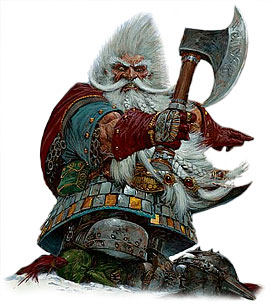
\includegraphics[width=6cm]{the-white-dwarf}
%\end{center}
%\end{figure}

\newpage
\textit{"Per aspera ad astra..."}

\pagebreak
\tableofcontents

\addcontentsline{toc}{chapter}{\protect\numberline{}Introduction}
\chapter{Introduction to the stars in high energy }

Let your imagination soar. 
By sitting on the old rocker looking at the sky with couple of good old whiskey you can easily 
start thinking about the universe. You are looking at a heck of a different kinds of cosmic 
objects, but suddenly you see almost only the stars. Almost all the shiny dots on the sky are 
stars and these stars are only the closest ones. Yes, you can see few other 
galaxies by naked eye\footnote{M31 and M33 in extremely good conditions on northern hemisphere
and Magellanic clouds on southern one}, but none of the exotic cosmic objects you are imaging about. 
They are too faint to be observed easily, because they are not only far, far away, but they also usually shine 
on different wavelengths, not visible by human eye.

Think about distances in the universe. One of the most accurate explanation is that from: \cite{hitch:1}  
\textit{"Space," it says, "is big. Really big. You just won't believe how vastly, 
hugely, mindbogglingly big it is. I mean, you may think it's a long way down the road to the 
chemist's, but that's just peanuts to space..."} 

Consider this, sometimes you want to study processes in these extreme, very faint objects, 
but they are too faint and too far in the universe. You are looking for “laboratory” with similar
 processes, but located much closer to the observer. The X-ray binary stars can be this kind 
of laboratories.  

There is, of course, many interesting phenomena which could be studied in X-ray binaries or in non-binary X-ray stars. 
Several of them are mentioned in the motivation section. 

I am mentioning many interesting things in this work, but the main effort is taken to 
study post shock region in the Intermediate Polars (IPs).   


\section{Motivation}
We can easily find many reasons why to study stars in the high energy bands.  
We can consider the direct and the most common scientific applications like observations of 
the supernovae, black holes \& neutron stars in X-ray binaries. But for the education purposes 
I prefer several others, very nice examples closer to topic of this work.  

\begin{itemize}
 \item \textbf{Relativistic jet phenomena}: like it was proposed by \citet{mirabel:1} that universal 
mechanism should be at work in all the relativistic jet sources in the universe. Better understanding 
of sources including: microblazars, AGNs and gamma-ray burst will help to gain more comprehensive 
understanding of these phenomena. Microblazars can play role of “space laboratories”, where interesting
 processes last on different timescales as is the case with AGNs or GRBs.   

\begin{figure}[!hbt]
\centering
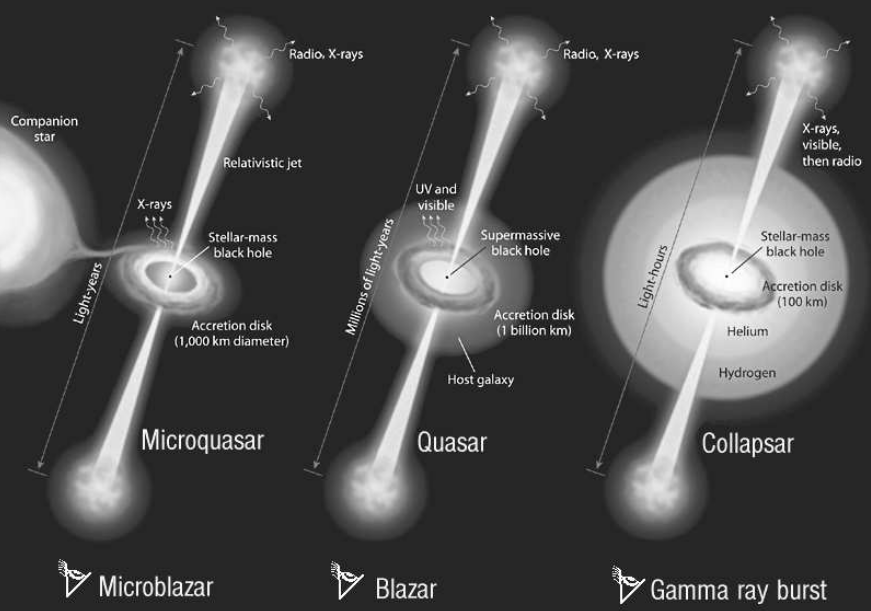
\includegraphics[totalheight=8.5cm]{microblazars}
\caption{NOT in scale diagram, showing curent ideas of micro-quasars, AGNs and gamma-ray
bursts as space objects driven by same, universal mechanism  \citet{mirabel:1}. }
\label{microblazar} 
\end{figure}

 \item \textbf{Galactic ridge X-ray emission (GRXE)}: various physical processes contribute to 
brightness of GRXE in different bands, but several studies in 3-20 keV provide evidence that diffuse 
X-ray radiation originates from huge number of stellar X-ray sources, mostly coronally active stars
 and white dwarf X-ray binaries. In particular for the energies over 20 keV to 200 keV is spectrum 
very similar to spectrum  of magnetic white dwarf binaries – e.g. Intermediate polars (IP) and polars (P).  
\citet{2007A&A...463..957K}
 
 \item \textbf{White dwarfs masses in Intermediate Polars (IP)}: as was proposed in \citet{1981ApJ...250..723R}, 
the temperature of the post shock region (PSR) depends on WD mass. Therefor the X-ray spectrum can be 
used for WD mass determination \citet{2005A&A...435..191S}. The WD mass estimations in cataclysmic stars 
is in general complicated. Usually the curve of radiation velocities can be used, but it is quit hard to constuct and
because of . 
Therefor X-ray spectrum method is very atractive for several reasons. This work is dedicated to this topic.  

\end{itemize}

\section{Aim of this work}
To cover the whole topic: ``stars in high energies'' is far behind capacity of such master thesis, because of that I decide 
to aim on cataclysmic variable stars (CVs), especialy to intermediate polars (IPs). 

As it will be mentioned in next sections closely, IPs are magnetized CVs where the compact, primary star 
is white dwarf with $B\sim 10^6 -10^7$ Gauss. The mass accretion is taking place from, mainly low-mass, non-degenerate star through Roche lobe.  
Accretion disk is in some distance from WD surface destroyed by strong magnetic field and 
accretion continuous through, so called, accretion curtain across magnetic force-field.

Falling material in some point creates stationary shock near the WD surface where the kinetic energy is converted 
through thermal bremsstrahlung to radiation. The temperature of such created plasma is typically more than 
10 keV with low density. The optically thin hard X-ray\footnote{In this case, hard X-rays means 10 - 120 keV region.} emission is taking place and heated gas creates 
post shock region (PSR) with temperature gradient. The hot gas then descends and cools by X-ray 
emission while it hits the WD surface.      

Because of relatively high temperature of PSR are IPs very good observed in hard X-rays band. 
IPs are only small fraction $\sim 15\%$ of all CVs, but they dominet in hard X-ray band over 10keV, ad most 
$\sim 80\%$ of detected CVs are IPs\citet{2009MNRAS.392..630L}. 

The temperature of PSR depends in first order only on WD mass, which is the most fundamental parameter of WDs.
This means, that if we are able to find temperature from fiting thermal bremsstrahlung model to spectrum of IP, 
we are also able to establis the WDs mass. 

An accrating WDs are very important for cosmology, because some of such objects probably casuse Type Ia supernovae, 
when the WD mass reaches Chandrasekhar limit. 

As is showed on figure~\ref{nylup1}, IP as NY Lup are well observed by INTEGRAL/IBIS detector which makes them 
iteresting space laboratories for WD basic parameters study. In same casesm, can by also accretion stream studied
if it is strong enough. 
    


\begin{figure}[!hbt]
\centering
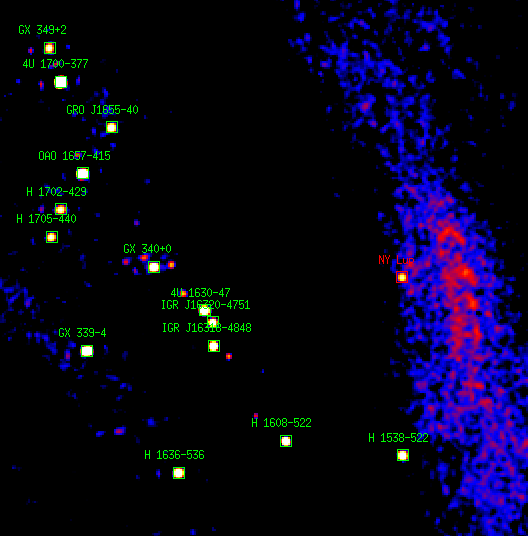
\includegraphics[totalheight=12cm]{plot/ds9_3}
\caption{1.2 Msec exposure of NY Lup region in 17-80 keV. The NY Lup is marked by red square. There are many others X-ray sources,
mostly HMXBs or LMXBs which is because of .}
\label{nylup1} 
\end{figure}



\section{Observations}
Cataclysmic Variable stars (CVs) have been, in fact, observed as early as ancient times. In historical 
records of  many civilizations we can find references for various astronomical events. Mostly they are 
about temporary objects: planets, Moon and Sun. However several are about comets and new stars. Rightly, 
these new stars are in many cases novae and supernovae. In China, the records date back to 1500 AD. 

Many records are saved from medieval time, for example positions of \textit{Nova Vulpecula 1670} and 
\textit{Nova Cygni 1600} (now knows as P Cygni) in Hevelius maps. 

With progress of astronomical photography in late 19th century started era of continuous observations
and with  development of first photo-multipliers in the mid-1940s CVs were begun attractive 
targets because of their big variability in different time scales. 

It is suitable to mention, that AAVSO has light curve of SS Cyg from 1896 up to date. 
\subsection{Optical and IR observations}
The very first visual observation was follows by photographic photometry and then spectroscopy, 
follows by photo-multiplier photometry since mid-1940s. The binary nature of all the CVs was confirm. 
The flickering was discovered and was assumed that it is somehow connected to stars duplicity Walker (1957),
\citet{warner:1}.

Statistical studies by Luyten and Hughes in mid-1960th showed, that novae remnants have $M_V \approx 4$ and 
dwarf novae at quisence have $M_V \approx 7.5$. They conculde that the hot primary star in CVs must by WD or 
 hot subdwarf \citet{warner:1}.   

The most important contribution of optical astronomy to this work is the discovery of large and 
variable circular polarization in several CVs. This helped to identified magnetic CVs, 
which were later divided to two categories, polars and intermediate polars.

There are more important discoveries in optical and IR bands in CVs subject. In case of interest the 
 \citet{warner:1} is proper book. 
   
   
\subsection{X-ray observations}
The very first CV detected in X-rays was the EX Hya observed by Uhuru X-ray space mission. 
Uhuru  works in 2.0 – 6.0 keV and in spite of its poor sensitivity the well-known 4U catalogue
 was created \citet{1978ApJS...38..357F} from its observations.

The NASA`s HEAO\footnote{High Energy Astronomy Observatory, The HEAO 2 was also known as 
The Einstein Observatory} program follows with three space missions. As the X-ray detectors 
technology evolves, the number of detected CVs grown linearly. \mbox{EXOSAT} provided long and 
uninterrupted data of many CVs during his operation from May 1983 until April 1986. 
Similar results were obtained from Soviet mission \mbox{Kvant 1} and Japan's Ginga.
The high hopes were entered into ROSAT which provides all-sky survey in the
 0.1 – 2.0 keV but expected huge number of new CVs was not discovered. 

The situation slightly changes with RXTE\footnote{Rossi X-ray Timing Explorer} which after 
years on orbit provides good data for several articles about WD masses \citet{2005A&A...435..191S}. 
The data from RXTE are used in new articles even $\sim15$ years after its launch \citet{2011A&A...526A..77B}.
 
Several others missions were launched in last ten years period. Few of them caried several 
detectors where one was sensitive in X-rays, like SUZAKU/XIS and Swift/XRT. But for the X-ray 
astronomy was been the year of 1999 the most important ever. The two major big observatories 
was launched on the Earth's orbit. The Chandra X-ray Observatory onboard STS-93 space shuttle 
Columbia on July and the XMM-Newton launched onboard ESA's Ariane 5 rocket.

   That was the beginning of the X-ray astronomy's golden era. During last decade the combination of 
Chandra and XMM provides enormous data archives which will be useful for astronomers for another 
decades. 

Sadly, there will not be such big observatory in X-rays for several decades. Only bigger space 
mission is Japan's ASTRO-H with several X-ray and gamma ray detectors on-board to cover broad 
high energy bands. The future of big ESA \& NASA space mission Athena (formerly: Constellation-X, 
XEUS, IXO)  is questionable because of budget cuts in both space agencies. 

Fortunately, there are several data archives with open data for anybody 
interested. This is big challenge mainly for young astronomers, who are 
not in any big space mission program but want to do science. In this case, 
they don't need any special hardware, even modern laptops are powerful enough.     



    
\subsection{Gamma ray observations}
In last millennium several space mission observed few CVs in bands from tents of keV to TeV.\footnote{The most 
studied CV from this era is AE Aqr (Meintjes 1990; Bowden et al. 1991)}
The biggest breakthrough came with ESA's INTEGRAL space mission which was able with its sensitivity 
and large field of view observed many CVs. Mostly intermediate polars. Only $\sim 2\%$ 
of all CVs are actually magnetic ones, but those ones are only visible in gamma rays.
INTEGRAL/IBIS was been used to determine white dwarf masses by \citet{2009MNRAS.392..630L}.

Two others space missions have on-board detectors similar to INTEGRAL/IBIS with their sensitivity 
and coverage: the NASA's Swift/BAT and Japan's Suzaku/XRT. Both are widely used to study white dwarf 
masses in IPs \citet{2009A&A...496..121B}, \citet{2010A&A...520A..25Y}.    



\chapter{White Dwarfs}
White dwarfs born when normall mass stars die. WDs are degenerated, late type stars with typical mass $\sim 1 M_{\odot}$. Their typical radius is about
 5000 km and mean density around $10^6 g.cm^{-3}$ \citet{2004bhwd.book.....S}. They no longer burn nuclear fuel and
if they don't have any other mather influx e.g. by accretion from close star, they slowly cools as they radiate
away residual thermal enegy.

WDs support themselves against gravity by the pressure of electron degenerate gas and theyr interior is in the local thermal 
equilibrium, except the thin atmosphere.  

\section{First look of white dwarfs interior}
WDs are a class of the less compact objects among the possible endpoints of the stellar evolution. 
The mass of the star is the main factor determining whether the star ends up as a WD, neutron star or a black hole.
The medium mass stars with masses $M \lesssim  4M_{\odot}$\footnote{Also $M \lesssim  8M_{\odot}$ can be find in 
some literature \citet{padm_vII}.} in some point of late state of their evolution gently spreads mass
 forming planetary nebulae. The rest of the star become the white dwarf.  

\begin{table}[hbt!]
\caption{Basic statisticks of the compact objects \citet{2004bhwd.book.....S}}
\centering
\begin{tabular}{lllll}
\hline
\hline
Object & Mass$^a$ & Radius$^b$ & Mean Density & Surface Potential  \\
       & $[M]$ & $[R]$ & $[r.cm^{-3}]$& $[GM/Rc^2]$                    \\
\hline
Sun         & $M_{\odot}$            & $R_{\odot}$             &1                  &$10^{-6}$ \\
White Dwarf & $\lesssim M_{\odot}$   & $\sim 10^{-2}R_{\odot}$ & $\lesssim 10^7$   &$\sim 10^{-4}$ \\
Neutron Star& $\sim1-3M_{\odot}$     & $\sim 10^{-5}R_{\odot}$ & $\lesssim 10^{15}$& $\sim 10^{-1}$\\
Black Hole  & Arbitrary              & $2GM/c^2$               & $\sim M/R^3$      & $\sim1$\\
\hline
\footnotesize
$^a M_{\odot}=1.989 \times 10^{33} g$ &&&& \\
\footnotesize
$^b R_{\odot}=6.9599 \times 10^{10} cm$ &&&& \\
\end{tabular}
\label{comobj1}
\end{table}

Let's use data from the table \ref{comobj1} and try to assume the pressure inside of WD. For very 
rough estimation, we can use equation of mechanic equilibrium to compare WD with the Sun.

\begin{equation}
 dP = -G\frac{M \varrho  dr}{r^2}
\end{equation}

The ratio between variables $P, M, \rho$ and $r$ in the Sun case and $P', M', \rho', r'$ in the WD's 
case can be written as follows:

\begin{center}
 $M' = M ,$  \\
 $r' = 10^{-2}r,$ \\
 $\rho' = 10^6 \rho,$ \\
\end{center}

From easy calculation we get: 
\begin{equation}
 dP' = -G\frac{M' \rho' dr'}{r'^2} = -G\frac{M \cdot 10^6 \rho \cdot 10^{-2} dr}{r^2 (10^{-2})^2} = 10^{8} dP
\end{equation}

From such results is eminent that there is something wrong with the WDs interior in comparation with central reion of the 
normal star. As the ionization is increasing by higher temperatures, the bigger pressure otherwise helps recombination. However 
very big pressure actually increase ionization up to totally ionized atoms. Atoms without their 
electrons shells are closer to each others which explains very high density.

For densities in range $10^5 gm.cm^{-3} \lesssim \rho \lesssim 10^9 gm.cm^{-3}$ the WD is made 
of ideal nondegenerate gas of ions and a degenerate gas of electrons. The system will be degenerate 
if $T>T_c$ where $T_c \approx 3 \times 10^9 K (\rho / \rho_c)^{2/3} $ 

If the electrons are relativistic or not can be found by comparing $m_e c$ with a fermi momentum
\begin{equation}
 p_F = (3\pi^2)^{1/3}\hbar n_e^{1/3} = (3\pi^2)^{1/3}\hbar (\rho/\mu_e)^{1/3}
\end{equation}
 where 
\begin{equation}
 \mu_e = (\rho / n_e m_p) = 2(1+X)^{-1}
\end{equation}
is the mass per electron. The fermi momentum will be equal to $m_e c$ at the critical density:
\begin{equation}
\rho_c \equiv \frac{8\pi}{3}m+p \mu_e \frac{m_ec^3}{h} \approx 10^6 \mu_e.gm.cm^{-3}
\end{equation}

If the density is higher than $\rho \gtrsim 10^9 gm.cm^{-3} $, the electrons are combined with protons inside of nuclei and 
create different matter called neutron degenerated gas. This is how neutron stars are made.    
 
\section{Fermi energy}
Now we can imagine interior of WDs as an area full of atoms nuclei very close to each other 
with free electrons around them. But electrons are fermions, which means that they must 
behave according to Pauli exclusion principle and it allows only at most one fermion 
per each quantum state. 

If we imagine a normal, everyday gas at standard temperature and pressure, only one 
of every $10^7$ quantum states is occupied by gas particles, so Pauli exclusion 
principle limitation is very insignificant. When energy is removed from the gas and 
it's temperature falls down, an increasingly large fraction of  the particles been 
forced into the lower energy states.

For fermions gas only one particle can take the lowest energy state and others must 
take another, higher and higher states, thus only one particle per state is allowed. 
Even in limit $T\rightarrow0$ pressure is produced by motions of electrons on excited positions.       

At the zero temperature all of the lowest states and none of the higher states are 
occupied, this kind of fermion gas is called completely degenerated. 
The max energy of electron in completely degenerate gas at $T=0 K$ is known as Fermi energy. 

For determining the limiting energy we can imagine 3D box where length of each of its sides will be \textit{L}.  
The wavelengths of electrons trapped in the box in each dimension will be
\begin{equation}
\lambda_{xyz} = \frac{2L}{N_{xyz}}
\end{equation}
where $N_{xyz}$ are integer quantum numbers for each dimension. The momentum can be written 
through de Broglie wavelength
\begin{equation}
p_{xyz} = \frac{hN_{xyz}}{2L}
\end{equation}
We can now write the total kinetic energy of the electron when $p^2 = p_x^2 + p_y^2 + p_z^2$ as follows
\begin{equation}
\label{ferm1}
 \varepsilon =  \frac{p^2}{2m} \Rightarrow \frac{h^2N^2}{8mL^2}
\end{equation}
Total number of electrons is same as total number of unique quantum numbers $N_x, N_y, N_z,$ multiply by 
factor two. The two factor comes from the fact that electrons are particles with spin, which can be $\pm 1/2$. 
This means that two electrons are allowed to have the same tree quantum numbers but different spin. 
The total number of electrons out to radius $N = \sqrt{N_x^2 + N_y^2 + N_z^2}$ will be
\begin{equation}
 N_e = 2\left ( \frac{1}{8} \right )\left ( \frac{4}{3} \pi N^3\right ) \Rightarrow N = \left ( \frac{3N_e}{\pi} \right )^{1/3} .
\end{equation}

By using Eq. \eqref{ferm1} and simplifying it, we will get the Fermi energy as follows
\begin{equation}
\varepsilon_F = \frac{\hbar^2}{2m}\left ( 3\pi^2n \right )^{2/3}
\end{equation}
where $m$ is the mas of the electron or any other fermion\footnote{Can by applies for any fermion, not only electrons} 
and $n\equiv N_e/L^3$ is the electron count per volume. 
The average energy per electron at $T = 0K$ is $\frac{3}{5}\varepsilon_F$.    
  
\section{Degeneracy}
Matter inside of WD has very symmetric spherical distribution, we can calculate the mass interior to radius $r$ like\footnote{More elaborate and precises approach can by find 
\citet{2004bhwd.book.....S}, \cite{padm_vII}, \citet{kleczek}, \citet{comp_obj1}, \citet{1972ApJ...175..417N} and simpler explanation with
less math in \citet{2007ima..book.....C}}
\begin{equation}
 \frac{dm_{(r)}}{dr} = 4 \pi r^2 \rho
\end{equation}
In normal case the WD is in steady state and gravitation force is balanced by the pressure at every point.  
For deriving the hydrostatic equilibrium equation we need to consider an infinitesimal element laying between 
$r$ and $r+dr$ with an area $dA$. The element is lying perpendicular to the radial direction, should looks like fig.(\ref{wd1}).
\begin{figure}[!hbt]
\centering
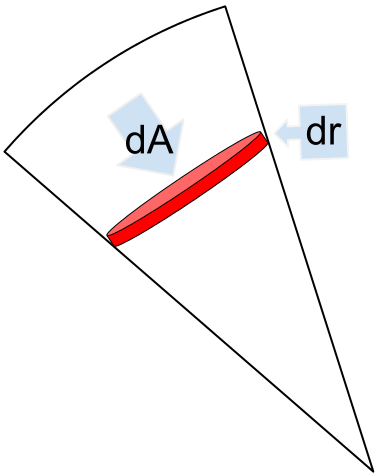
\includegraphics[totalheight=4cm]{plot/wd1}
\caption{How could be infinitesimal fluid element laying between 
$r$ and $r+dr$ with an area $dA$ imagine}
\label{wd1} 
\end{figure}

The gravitation attraction between mass $dm = \rho dA dr$ and $m_{(r)}$ is the same as if $m_{(r)}$ were only point at the center with the same mass. While the outside mass exerts no force on $dm$.
Then the net outward pressure forced on $dm$ is $- \left [ P\left ( r + dr \right ) - p(r)  \right ]dA$. In equilibrium 
\begin{equation}
\label{eq1}
 \frac{dP}{dr} = - \frac{Gm_{(r)}\rho}{r^2}
\end{equation}
In such equilibrium, the gradient of degeneracy pressure is balanced by gravitation: 
\begin{equation}
\label{equ_1}
\nabla P = -\rho \nabla \Phi, 
\end{equation}
where $\Phi$ means gravitation potential.  
Consequence of the Eq.\eqref{eq1} is the viral theorem. The gravitation potential energy of the star is then 
\begin{equation}
\label{pot_e_star1}
W = -\int_{0}^{R} \frac{Gm_{(r)}}{r}\rho 4 \pi r^2 dr = \int_{0}^{R} \frac{dP}{dr}4\pi r^3 dr = -3\int_{0}^{R} P4 \pi r^2 dr
\end{equation}
We can characterize the gas by an adiabatic equation of state, where $K$ and $\Gamma$ are constants
\begin{equation}
 \label{adiab_1}
P = K\rho_0^\Gamma
\end{equation}
Then Eq.\eqref{pot_e_star1} can be rewritten as follows
\begin{equation}
 W = -3 (\Gamma - 1) U,
\end{equation}
Where $U$ is the total star's internal energy 
\begin{equation}
U = \int_{0}^{R}\varepsilon' 4\pi r^2 dr 
\end{equation}
and $\varepsilon'$ comes from:
\begin{equation}
\label{eps1}
 \varepsilon' \equiv \varepsilon - \rho_0 c^2
\end{equation}
where
\begin{equation}
 \varepsilon = \rho_0c^2+\frac{P}{\Gamma -1}
\end{equation}
Now we can see that the energy density, of the gas (excluding the rest mass energy) can be also written as
\begin{equation}
 \label{eps2}
 \varepsilon'=\frac{P}{\Gamma - 1}
\end{equation}
Assuming adiabatic changes, the Eq.\eqref{eps2} follows from the first law of thermodynamics
\begin{equation}
 d\left ( \frac{\varepsilon }{\rho_0} \right ) = -Pd\left ( \frac{1}{\rho_0} \right ) .
\end{equation}

The equation of state for ideal Fermi gas reduce to the simple polytropic form Eq.\eqref{adiab_1} in
the two limiting cases \citet{2004bhwd.book.....S}, \citet{padm_vII}:
\begin{itemize}
\item Nonrelativistic electrons, $\rho_0 \ll 10^6 g.cm^{-3}, x\ll 1, \Phi_{(x)}\rightarrow x^5/15\pi^5 $
\begin{equation}
\Gamma = \frac{5}{3} \Longrightarrow  K = \frac{3^{\frac{2}{3}}\pi^{\frac{4}{3}}}{5}\frac{\hbar^2}{m_em_u^{\frac{5}{3}}u_e^{\frac{5}{3}}} = \frac{1.0036\times 10^{13}}{u_e^{\frac{5}{3}}} cgs.
\end{equation}
\item Extremly relativistic electrons, $\rho_0 \gg 10^6 g.cm^{-3}, x\gg 1, \Phi_{(x)}\rightarrow x^4/12\pi^2 $
\begin{equation}
\Gamma = \frac{4}{3} \Longrightarrow K = \frac{3^{\frac{1}{3}}\pi^{\frac{2}{3}}}{4}\frac{\hbar c}{m_u^{\frac{4}{3}}u_e^{\frac{4}{3}}} = \frac{1.2435\times 10^{15}}{u_e^{\frac{4}{3}}} cgs.
\end{equation}
\end{itemize}

This kind of the equilibrium configurations such these are called polytropes. We can use Eq.\eqref{equ_1}, take the divergence of it and by using $\nabla^2\Phi = 4\pi G \rho$ in spehrically 
symmetric case we get  
\begin{equation}
\label{pol_1}
 \frac{1}{r^2}\frac{d}{dr}\left ( \frac{r^2}{\rho}\frac{dP}{dr} \right ) = -4\pi G\rho .
\end{equation}
Using few trics, Eq.\eqref{pol_1} can be rewrite and reduce to dimension less form 
\begin{equation}
 \label{pol_2}
\frac{1}{\xi^2 }\frac{d}{d\xi}\xi^2\frac{d\theta }{d\xi } = -\theta^n 
\end{equation}



use Eq.\eqref{adiab_1} with $\Gamma \equiv 1 + \frac{1}{n}$ where $n$ is called the polytropic index
\begin{equation}
\label{pol_3}
\rho = \rho_c \theta^n  
\end{equation}
\begin{equation}
\label{pol_4}
r = a\xi
\end{equation}
\begin{equation}
\label{pol_5} 
a = \left [ \frac{\left ( n+1 \right ) K \rho_c^{\left ( 1/n-1 \right )} }{4\pi G} \right ]^{1/2}
\end{equation}
where $\rho_c$ is the central density, $\rho_c = \rho$ when $r = 0$. 

The Eq.\eqref{pol_2} is called the \textit{Lane-Emden equation} for the structure of $n$ index, the boundary 
conditions at the center such polytropic white dwarf are
\begin{equation}
\label{le1}
 \theta(0) = 1, 
\end{equation}
\begin{equation}
\label{le0}
 \theta'(0)= 0.
\end{equation}
The condition \eqref{le1} come dirrectly from Eq.\eqref{pol_3} and condition \eqref{le0} is derived from the fact 
that near the center of the star is $m_{(r)} \approx 4\pi \rho_c \frac{r^3}{3}$. If we use Eq.\eqref{eq1}, we get
\begin{equation}
 \frac{dP_{(\rho)}}{dr} = \frac{d\rho}{dr} = 0 .
\end{equation}

If we numerically integrate Eq.\eqref{pol_2} using Eq.\eqref{le1} and Eq. \eqref{le0} as the boundary conditions, 
starting at $\xi=0$. We will find that for $n<5$ $(Gamma>\frac{6}{5})$ this solution decrease monotonically with a zero 
at finite value $\theta(\xi_1) = 0$, which corresponds to the star's surface where $P=\rho = 0$ and we get the 
equation for white dwarf radius 
\begin{equation}
 \label{radius1}
R = a\xi_1 = \left[ \frac{(n+1)K}{4\pi G} \right]^{1/2}\rho_c^{\frac{1-n}{2n}}\xi_1.
\end{equation}

The mass o thef WD can be find as follows
\begin{equation}
 \label{wdmass}
\begin{split}
M &= \int_{0}^{R} 4\pi r^2 \rho dr \\
  &= 4 \pi a^3 \rho_c \int_{0}^{\xi_1} \xi^2 \theta^n d\xi \\
  &= -4 \pi a^3 \rho_c \int_{0}^{\xi_1}\frac{d}{d\xi}\left( \xi^2 \frac{d\theta}{d\xi}\right)d\xi \\
  &= 4 \pi a^3 \rho_c \xi_1^2 \lvert \theta' (\xi_1) \lvert \\
  & = 4 \pi \left[ \frac{(n+1)K}{4 \pi G}\right]^{3/2} \rho_c^{\frac{(3-n)}{2\pi}}\xi_1^2 \lvert \theta' (\xi_1)\lvert ,
\end{split}
\end{equation}
then $\rho_c$ can by eliminated between Eq.\eqref{radius1} and Eq.\eqref{wdmass}, which gives the mass-radius relations 
for polytropes \citet{2004bhwd.book.....S}:  
\begin{equation}
\label{mr_eq}
 M = 4 \pi R^{\frac{3-n}{t-n}}\left[ \frac{(n+1)K}{4 \pi G}\right]^{\frac{n}{n-1}}
\xi_1^{\frac{3-n}{1-n}}\xi_1^2\lvert\theta' (\xi_1) \lvert
\end{equation}

\section{The Chandrasekhar limit}
What will happen if $\rho_c \rightarrow \infty$? This is one of the most important questions in the universe. 
Because how central density of WD increases by increase of the WD mass, the electrons become more and more 
relativistic throughout the star. As $R\rightarrow 0 $ also the space for free electrons moving between atoms nuclei become
smaller and smaller. With increasing mass must also increase the speed of electrons to support the degeneracy pressure.  
While the mass of WD is larger the radius become smaller, mass-volume relations implies that $\rho\propto M_{WD}^2$. 
But the electrons can't have speed larger than speed of light and in some point where $\rho \sim 10^9 g cm ^{-3}$ there 
will be no space left for moving electrons and they will be press into the nuclei. This will leads to explosion of such WD. 

\begin{figure}[hbt!]
\centering
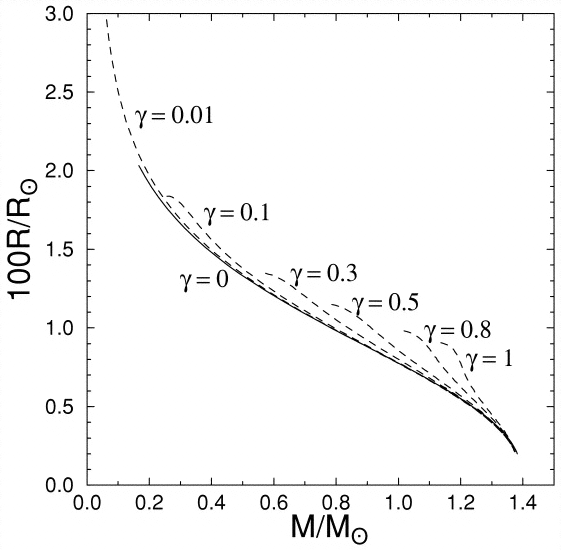
\includegraphics[totalheight=8cm]{plot/chlimit}
\caption{Relation between the mass $M$ and radius $R$ of a $^{12}C$ magnetic white dwarf for the indicated magnetic field strengths. 
The solid line denotes the \citet{1961ApJ...134..683H} model for nonmagnetic white dwarfs $(\gamma = 0)$. The dashed lines are magnetic 
white dwarfs. \citet{2000ApJ...530..949S} }
\label{Chlimit1} 
\end{figure}

This all means, that there is a maximum mass for WDs. This mass is called \textit{Chandrasekhar limit}
\footnote{Named after Indian physicist Subrahmanyan Chandrasekhar who received the Nobel Price in Physics in 1983 for his 
work on stellar structure and evolution. Chandrasekhar made his great discovery at the age of 21 in the 1931.   } $M_{ch}$.  

The classical theory of type 1A supernovae assumes explosions of such WDs reaching the $M_{ch}$, the very same 
mass of the WDs when they explode makes Type 1A supernovae perfectly suitable objects for measuring the long range 
space distances. That's why they are so important objects for cosmology and astronomers called 
them standard candles.

The Chandrasekhar limit for relativistic electron case is
\begin{equation}
 \label{chlim}
M=1.457\left ( \frac{2}{\mu_e} \right )^2 M_{\odot},
\end{equation}
where $\mu_e$ is the average molecular weight per electron, which depends on the chemical comsposition of the star and is typically sets 
to $\mu_e = 2$. 

The Eq.\eqref{chlim} can be obtained by solving Eq.\eqref{mr_eq} with parameters\footnote{Extensive list of polytropic parameters can be find in
\citet{1939MNRAS..99..673C}}:
\begin{equation}
\Gamma = \frac{4}{3}, n =3,{   }\xi_1 = 6.89685, \xi_1^2 \lvert \theta' (\xi_1) \lvert = 2.01824. 
\end{equation}
                                                                                                                                                                                                                                                                                                                                                                                                                                                                                                                                                                                                                                                                                                                                                                                                                                                                                                                                                                                                                                                                                                                                                                                                                                                                                                                                                                                                                                                                                                                                                                                                                                                                                                                                                                                                                                                                                                                                                                                                                                                                                                                                                                                                                                                                                                                                                                                                                                                                                                                                                                                                                                                                                                                                                                                                                                                                                                                                                                                                                                                                                                                                                                                                                                                                                                                                                                                                                                                                                                                                                                                                                                                                                                                                                                                                                                                                                                                                                                                                                                                                                                                                                                                                                                                                                                                                                                                                                                                                                                                                                                                                                                                                                                                                                                                                                                            
Another, ilustrativ aproach to estimating the Chandrasekhar limit is mention in \citet{2007ima..book.....C}. An approximate value for $M_{ch}$ may by 
obtain by setting the estimate of the central pressure
\begin{equation}
 P_c \approx \frac{2}{3} \pi G \rho^2 R_{wd}^2 \qquad \text{with} \qquad \rho=M_{wd} / \frac{4}{3} \pi R_{wd}^3  
\end{equation}
equal to electron degeneracy pressure equation
\begin{equation}
 \label{edegP}
P = \frac{(3\pi^2)^{2/3}}{4} \hbar c \left[ \left( \frac{Z}{A}\right) \frac{\rho}{m_H}\right]^{4/3},
\end{equation}
with $\frac{Z}{A}=0.5$, the $R$ cancels from the equation leving for the greatest possible mass:
\begin{equation}
 \label{chlim2}
M_{ch} \sim \frac{3\sqrt{2\pi}}{8}\left ( \frac{\hbar c}{G} \right )^{3/2}\left [ \left ( \frac{Z}{A} \right ) \frac{1}{m_H} \right ]^2 M_\odot.  
\end{equation}
It is important to notice that Eq.\eqref{chlim2} contains three fundamental constants $\hbar, c$ and $G$ representing the combined effects of quantum mechanics, 
relativity and Newtonian gravitation on the WD structure. 

The Chandrasekhar limit slightly depends upon the chemical composition \eqref{chlim}, but in the literature is well known as $M_{ch} = 1.44M_\odot$.    
  
The similar limit exists for neutron stars, where pressure of degenerate neutron gas support the stars against it own gravity. 
This limit is called Tolman - Oppenheimer - Volkoff limit (or TOV limit).But it is not so easy in neutron stars case. Their limit 
mass depends strongly on type of matter in star center. The limit varies from $0.7 M_\odot$ up to $\sim 3M_\odot$ in extreme case, when inner section of 
neutron star is partialy filled up by quark - gluon meatter.     


\section{White dwarfs classes}
Previous sections describe interior and fundamental parameters of white dwarfs, but it also important to tell something about their classes.   
WDs occupy narrow sliver line in the left bottom corner of H-R diagram fig.(\ref{hrd1}), slightly parallel with the main sequence.  
Although WDs are typically whiter then normal stars, the name itself is not very comprehensive. WD in fact come in all colors with surface 
temperatures from less than $4000K$ to even more than $80,000K$. The $D$ for \textit{dwarf} spectral type has several subdivisions:
\begin{itemize}
 \item \textbf{DA} white dwarfs is the largest group $(\sim 60\%)$ including Sirius B, their spectra have only pressure-broadened hydrogen lines 
 \item \textbf{DB} white dwarfs $(\sim 8\%)$ have only helium absorbtion lines in their spectra 
 \item \textbf{DC} white dwarfs $(\sim 14\%)$ have no lines, but only continuum features
 \item \textbf{DQ} white dwarfs show carbon features in their spectra
 \item \textbf{DZ} white dwarfs show some evidence of metal lines
\end{itemize}

Very small radius makes WDs hard to observed in optical band. The brightest and also the most known WD is Sirius B with visual magnitude $\sim8.6$. 
Unfortunately it is located only $8”$ from his companion Sirius A, the brightness star of the night sky. Although the WD are not common stars 
on the  night sky, their are not rare in our Galaxy. From hundred closes stars to our Sun, eight of them are WDs.

WDs usually have very strong magnetic field which comes from weak surface magnetic field of progenitor's star which lagre surface are conserved to their very 
small surfaces. The magnetic field intensities vary from about $1000 gauss$ up to $10^9 gauss$ in extreme cases.    

WDs can by find alone in interstellar space, young ones can be find also in planetary nebulae, like one  in center of the Ring nebula 
M57 or their can be find in cataclysmic variables.       
 
\begin{figure}[hbt!]
\centering
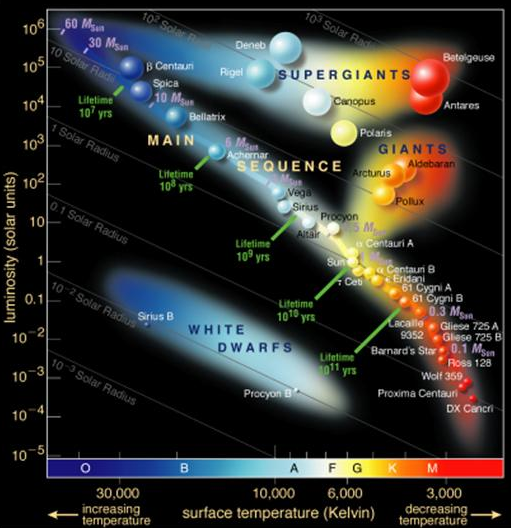
\includegraphics[totalheight=12cm]{hrdiagram}
\caption{WD lies in right bottom corner of HD diagram, under main 
sequence, which exactly means, they are very small (dwarf) stars with high surface temperature.  }
\label{hrd1} 
\end{figure}


\chapter{Cataclysmic variable stars}
\section{Non magnetic cataclysmic variables} 
\section{Magnetic cataclysmic variables}
\subsection{Polars}
\subsection{Intermediate polars}
\section{Galactic population ofcataclysmic variables }
\section{Others important creatures}
\section{GXRE}



\chapter{Masses of white dwarfs in intermediate polars}
\section{Breaking radiation}
\subsection{Bremsstrahlung}
\begin{equation}
 a_{\parallel} = \dot{v}_x = -\frac{eE_x}{m_e}\frac{\gamma {Z_e}^2 vt}{4\pi \varepsilon_0 m_e \left [ b^2 + \left ( \gamma vt \right )^2  \right ]^{2/3}} 
\end{equation}

\subsection{Thermal bremsstrahlung}



\section{Synchrotron radiation}
\section{Post shock region}
\section{WD mass estimations methods}

\chapter{Data analysis}

\section{INTEGRAL}

\begin{figure}[!hbt]
\centering
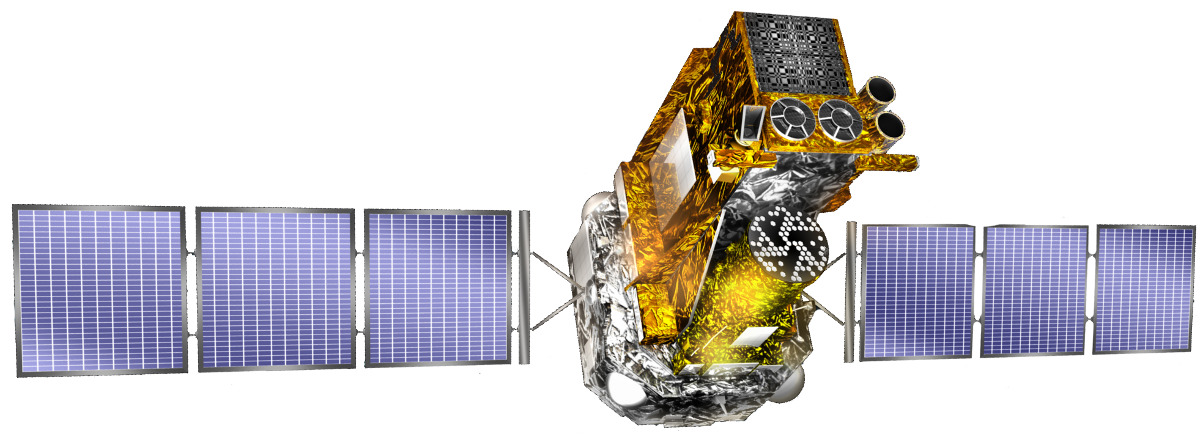
\includegraphics[totalheight=4cm]{integral}
\caption{INTEGRAL}
\label{microblazar} 
\end{figure}


\section{XMM-Newton}

\begin{figure}[!hbt]
\centering
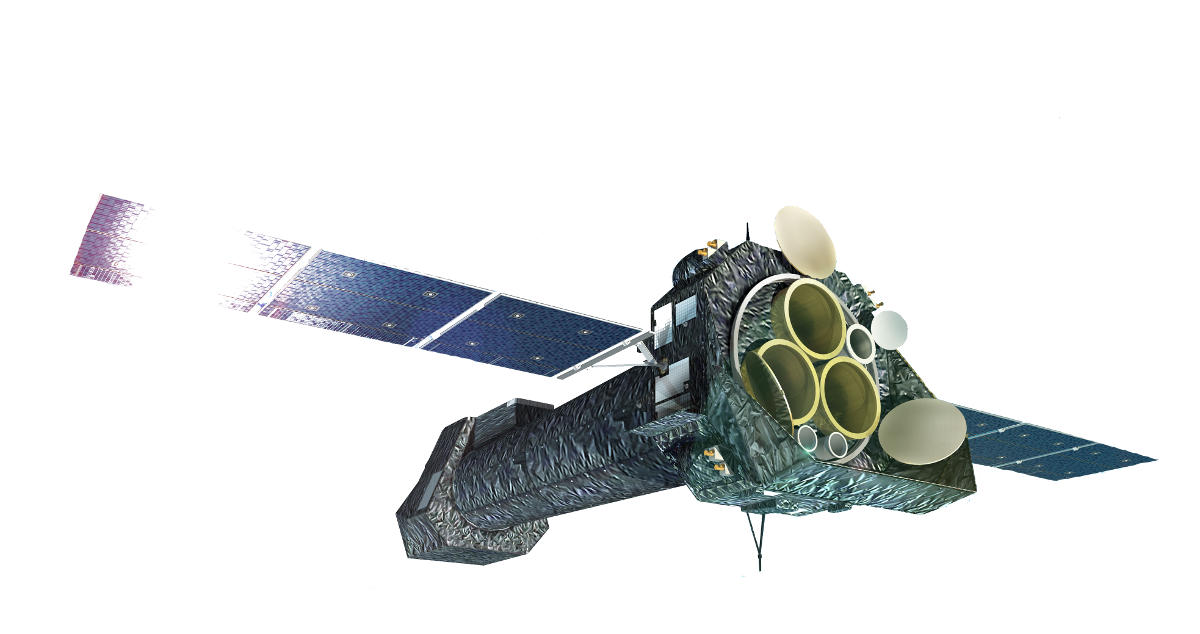
\includegraphics[totalheight=6cm]{XMM}
\caption{XMM-Newton }
\label{microblazar} 
\end{figure}


\section{Results}
\section{Discussion}
\chapter{Conclusions}



%\section{Hmotnosť bieleho trpaslík}
%\subsection{Pomocou kontinua}
%\subsection{Pomocou K železných čiar}
%\chapter{Spracovanie dát}
%\section{INTEGRAL}
%\section{XMM-Newton}
%\chapter{Určenie hmotností vybraných IP}



%\chapter{Intermedialne polary}   

\nocite{2004bhwd.book.....S}
\nocite{2009A&A...496..121B}
\nocite{accpower:1}
\nocite{2005A&A...435..191S}
\nocite{2008A&A...489.1121R}
\nocite{2010A&A...520A..25Y}
\nocite{warner:1}
\nocite{2006A&A...450..117S}
\nocite{rybicki:1}
\nocite{1973PThPh..49.1184A_aizu}
\nocite{astrop_techniques_5th}
\nocite{xray_hanbook}
\nocite{1972ApJ...175..417N}
\nocite{kleczek}
\nocite{comp_obj1}
\nocite{1939MNRAS..99..673C}
\bibliography{koci}
\addcontentsline{toc}{chapter}{\hspace*{6mm}Bibliography}



\clearpage

\appendix
\section*{Appendix}
\addcontentsline{toc}{chapter}{\hspace*{6mm}Apendix}
this will be the appendix
%\pagebreak



\begin{sidewaystable}
\begin{center}
 

\caption{Estimated WD masses from previous reports ...}
\begin{tabular}{llllllll}
\hline
\hline
%\multicolumn{2}{c}{Item} \\
System & Suzaku & Swift & RXTE & RXTE & Ginga & ASCA& This work  \\
       & XIS+HXD & BAT& PCA+HEXTE & PCA & LAC & SIS & XMM \& Integral                     \\
       & $M_{WD}$ &$M_{WD}$ &$M_{WD} $&$M_{WD}$ &$M_{WD}$ &$M_{WD}$ &$M_{WD}$ \\
\hline
 FO Aqr      &         &        &          &     &      &         &           \\
 XY Ari      &         &        &          &     &      &         &           \\
 MU Cam      &         &        &          &     &      &         &           \\
 BG CMi&         &        &          &     &      &         &           \\
 V709 Cas&         &        &          &     &      &         &           \\
 TV Col&         &        &          &     &      &         &           \\
 TX Col&         &        &          &     &      &         &           \\
 YY Dra&         &        &          &     &      &         &           \\
 PQ Gem&         &        &          &     &      &         &           \\
 EX Hya&         &        &          &     &      &         &           \\
 NY Lup&         &        &          &     &      &         &           \\
 V2400 Oph&         &        &          &     &      &         &           \\
 AO Psc&         &        &          &     &      &         &           \\
 V1223 Sgr&         &        &          &     &      &         &           \\
 RX J2133&         &        &          &     &      &         &           \\
 IGR J17303&         &        &          &     &      &         &           \\

\hline
\end{tabular}

\end{center}
\end{sidewaystable}
%\thispagestyle{empty}
%\LaTeX{}
\end{document}


